\iffalse
\let\negmedspace\undefined
\let\negthickspace\undefined
\documentclass[journal,12pt,twocolumn]{IEEEtran}
\usepackage{cite}
\usepackage{amsmath,amssymb,amsfonts,amsthm}
\usepackage{algorithmic}
\usepackage{graphicx}
\usepackage{textcomp}
\usepackage{xcolor}
\usepackage{txfonts}
\usepackage{listings}
\usepackage{enumitem}
\usepackage{mathtools}
\usepackage{gensymb}
\usepackage[breaklinks=true]{hyperref}
\usepackage{tkz-euclide} % loads  TikZ and tkz-base
\usepackage{listings}



\newtheorem{theorem}{Theorem}[section]
\newtheorem{problem}{Problem}
\newtheorem{proposition}{Proposition}[section]
\newtheorem{lemma}{Lemma}[section]
\newtheorem{corollary}[theorem]{Corollary}
\newtheorem{example}{Example}[section]
\newtheorem{definition}[problem]{Definition}
%\newtheorem{thm}{Theorem}[section] 
%\newtheorem{defn}[thm]{Definition}
%\newtheorem{algorithm}{Algorithm}[section]
%\newtheorem{cor}{Corollary}
\newcommand{\BEQA}{\begin{eqnarray}}
\newcommand{\EEQA}{\end{eqnarray}}
\newcommand{\define}{\stackrel{\triangle}{=}}
\theoremstyle{remark}
\newtheorem{rem}{Remark}
%\bibliographystyle{ieeetr}
\begin{document}
%
\providecommand{\pr}[1]{\ensuremath{\Pr\left(#1\right)}}
\providecommand{\prt}[2]{\ensuremath{p_{#1}^{\left(#2\right)} }}        % own macro for this question
\providecommand{\qfunc}[1]{\ensuremath{Q\left(#1\right)}}
\providecommand{\sbrak}[1]{\ensuremath{{}\left[#1\right]}}
\providecommand{\lsbrak}[1]{\ensuremath{{}\left[#1\right.}}
\providecommand{\rsbrak}[1]{\ensuremath{{}\left.#1\right]}}
\providecommand{\brak}[1]{\ensuremath{\left(#1\right)}}
\providecommand{\lbrak}[1]{\ensuremath{\left(#1\right.}}
\providecommand{\rbrak}[1]{\ensuremath{\left.#1\right)}}
\providecommand{\cbrak}[1]{\ensuremath{\left\{#1\right\}}}
\providecommand{\lcbrak}[1]{\ensuremath{\left\{#1\right.}}
\providecommand{\rcbrak}[1]{\ensuremath{\left.#1\right\}}}
\newcommand{\sgn}{\mathop{\mathrm{sgn}}}
\providecommand{\abs}[1]{\left\vert#1\right\vert}
\providecommand{\res}[1]{\Res\displaylimits_{#1}} 
\providecommand{\norm}[1]{\left\lVert#1\right\rVert}
%\providecommand{\norm}[1]{\lVert#1\rVert}
\providecommand{\mtx}[1]{\mathbf{#1}}
\providecommand{\mean}[1]{E\left[ #1 \right]}
\providecommand{\cond}[2]{#1\middle|#2}
\providecommand{\fourier}{\overset{\mathcal{F}}{ \rightleftharpoons}}
\newenvironment{amatrix}[1]{%
  \left(\begin{array}{@{}*{#1}{c}|c@{}}
}{%
  \end{array}\right)
}
%\providecommand{\hilbert}{\overset{\mathcal{H}}{ \rightleftharpoons}}
%\providecommand{\system}{\overset{\mathcal{H}}{ \longleftrightarrow}}
	%\newcommand{\solution}[2]{\textbf{Solution:}{#1}}
\newcommand{\solution}{\noindent \textbf{Solution: }}
\newcommand{\cosec}{\,\text{cosec}\,}
\providecommand{\dec}[2]{\ensuremath{\overset{#1}{\underset{#2}{\gtrless}}}}
\newcommand{\myvec}[1]{\ensuremath{\begin{pmatrix}#1\end{pmatrix}}}
\newcommand{\mydet}[1]{\ensuremath{\begin{vmatrix}#1\end{vmatrix}}}
\newcommand{\myaugvec}[2]{\ensuremath{\begin{amatrix}{#1}#2\end{amatrix}}}
\providecommand{\rank}{\text{rank}}
\providecommand{\pr}[1]{\ensuremath{\Pr\left(#1\right)}}
\providecommand{\qfunc}[1]{\ensuremath{Q\left(#1\right)}}
	\newcommand*{\permcomb}[4][0mu]{{{}^{#3}\mkern#1#2_{#4}}}
\newcommand*{\perm}[1][-3mu]{\permcomb[#1]{P}}
\newcommand*{\comb}[1][-1mu]{\permcomb[#1]{C}}
\providecommand{\qfunc}[1]{\ensuremath{Q\left(#1\right)}}
\providecommand{\gauss}[2]{\mathcal{N}\ensuremath{\left(#1,#2\right)}}
\providecommand{\diff}[2]{\ensuremath{\frac{d{#1}}{d{#2}}}}
\providecommand{\myceil}[1]{\left \lceil #1 \right \rceil }
\newcommand\figref{Fig.~\ref}
\newcommand{\systemL}[1]{\stackrel{#1}{\xleftrightarrow{\mathcal{L}}}}
\newcommand{\systemLinv}[1]{\stackrel{#1}{\xleftrightarrow{\mathcal{L}^{-1}}}}


\newcommand\tabref{Table~\ref}
\newcommand{\sinc}{\,\text{sinc}\,}
\newcommand{\rect}{\,\text{rect}\,}
%%
%	%\newcommand{\solution}[2]{\textbf{Solution:}{#1}}
%\newcommand{\solution}{\noindent \textbf{Solution: }}
%\newcommand{\cosec}{\,\text{cosec}\,}
%\numberwithin{equation}{section}
%\numberwithin{equation}{subsection}
%\numberwithin{problem}{section}
%\numberwithin{definition}{section}
%\makeatletter
%\@addtoreset{figure}{problem}
%\makeatother

%\let\StandardTheFigure\thefigure
\let\vec\mathbf


\bibliographystyle{IEEEtran}
\title{ GATE NM-54 2022}
\author{EE23BTECH11011- Batchu Ishitha$^{*}$% <-this % stops a space
}
\maketitle




\bigskip

\renewcommand{\thefigure}{\theenumi}
\renewcommand{\thetable}{\theenumi}
%\renewcommand{\theequation}{\theenumi}

Q: A system with two degrees of freedom, as shown in the figure, has masses $m_1=200kg$ and $m_2=100kg$ and stiffness coefficients $k_1=k_2=200N/m$. Then the lowest natural frequency of the system is  \underline{\hspace{2.5cm}} rad/s (rounded off to one decimal place).    
\begin{figure}[!ht]
    \centering
    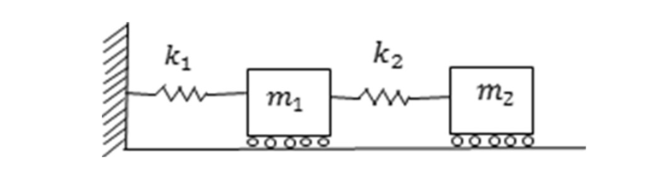
\includegraphics[width=\columnwidth]{2022/NM/54/figs/g54.fig1.png}
    \caption{ }
    \label{fig:ishitha.g22.nm.54.f1}
\end{figure}                   
\\    \hfill{GATE NM 2022} \\

\solution
\fi

\begin{figure}[!ht]
    \centering
    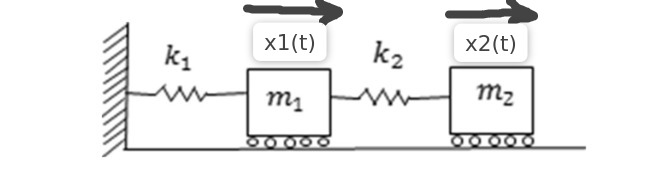
\includegraphics[width=\columnwidth]{2022/NM/54/figs/g54.fig2.jpeg}
    \caption{ }
    \label{fig:ishitha.g22.nm.54.f2}
\end{figure} 

METHOD-1:

\begin{table}[!ht]    
    \centering
    \resizebox{9cm}{2cm}{
            \begin{tabular}{|c|c|c|} 
    \hline
\textbf{Variable} & \textbf{Description} & \textbf{Value} \\\hline
    $m_1$ & Mass of block 1 & $200kg$  \\\hline
    $m_2$ & Mass of block 2 & $100kg$  \\\hline
    $k_1$ & Stiffness coefficient of spring$1$ & $200N/m$  \\\hline
    $k_2$ & Stiffness coefficient of spring$2$ & $200N/m$  \\\hline
        \end{tabular}
    
        
 
    }
    \caption{Input Parameters}
    \label{table:ishitha.g22.nm.54.t1}
\end{table}


\begin{align}
m_1\ddot{x_1}(t) - k_2\brak{x_2(t)-x_1(t)}+ k_1x_1(t)&=0
\label{eq:ishitha.g22.nm.54.1.eq}\\
m_2\ddot{x_2}(t) + k_2\brak{x_2(t)-x_1(t)}&=0
\label{eq:ishitha.g22.nm.54.2.eq} 
\end{align}

Writing ~\eqref{eq:ishitha.g22.nm.54.1.eq} and ~\eqref{eq:ishitha.g22.nm.54.2.eq} in matrix form:
\begin{align}
\myvec{
m_1 & 0  \\
0 & m_2
}
\myvec{
\ddot{x_1}(t) \\
\ddot{x_2}(t)
}
+
\myvec{
k_1+k_2 & -k_2  \\
-k_2 & k_2
}
\myvec{
x_1(t) \\
x_2(t)
}
=
\myvec{
0 \\
0
}
\end{align}

\begin{equation}
x(t)     \systemL{}   X(s)  
\end{equation}


\begin{equation}
x^{''}(t) \systemL{} s^{2}X(s)-sx(0)-x^{'}(0)
\end{equation}

Applying Laplace transform for ~\eqref{eq:ishitha.g22.nm.54.1.eq} and ~\eqref{eq:ishitha.g22.nm.54.2.eq} \\ assuming they are at their repective maximum displacement at t=0 
\begin{align}
m_1\brak{s^2X_1(s) -sx_1(0)-0} - k_2\brak{X_2(s)-X_1(s)} + k_1X_1(s) &= 0
\label{eq:ishitha.g22.nm.54.3.eq} \\
m_2\brak{s^2X_2(s)-sx_2(0)-0} + k_2\brak{X_2(s)-X_1(s)}&=0
\label{eq:ishitha.g22.nm.54.4.eq} 
\end{align}

Writing ~\eqref{eq:ishitha.g22.nm.54.3.eq} and ~\eqref{eq:ishitha.g22.nm.54.4.eq} in matrix form:
\begin{align}
\myvec{
m_1s^2+(k_1+k_2) & -k_2  \\
-k_2& m_2s^2+k_2
}
\myvec{
X_1(s) \\
X_2(s)
}
=
\myvec{
m_1sx_1(0) \\
m_2sx_2(0)
}
\end{align}

\begin{align}
\myvec{
X_1(s) \\
X_2(s)
}
= \frac{1}{m_1m_2s^4+(k_1+k_2)m_2s^2+k_2m_1s^2+k_1k_2} 
\myvec{
m_2s^2+k_2 & k_2  \\
k_2& m_1s^2+(k_1+k_2)
}
\myvec{
m_1sx_1(0) \\
m_2sx_2(0)
}
\end{align}

\begin{align}
\implies X_1(s)&=\frac{m_1m_2s^3x_1(0)+k_2m_1sx_1(0)+m_2k_2sx_2(0)}{m_1m_2s^4+(k_1+k_2)m_2s^2+k_2m_1s^2+k_1k_2} \\
\implies X_2(s)&=\frac{m_1k_2sx_1(0)+m_1m_2s^3x_2(0)+(k_1+k_2)m_2sx_2(0)}{m_1m_2s^4+(k_1+k_2)m_2s^2+k_2m_1s^2+k_1k_2}
\end{align}

Considering denominator of $X_i(s)$ for $i=1,2$(ie: characteristic equation of the system):
\begin{align}
m_1m_2s^4+(k_1+k_2)m_2s^2+k_2m_1s^2+k_1k_2 &=0 \\
s^4 +4s^2+2&=0\\
\implies s^2&=\frac{-4\pm \sqrt{16-8}}{2} \\
&= -2 \pm \sqrt{2} 
\end{align}
The roots of s are imaginary so it's Sinusoid.
\begin{align}
\omega&=\pm\sqrt{2\mp \sqrt{2}}\\
\implies \omega_{least} &= 0.765 rad/s
\end{align} 


METHOD-2:CONVERTING MECHANICAL SYSTEM INTO ITS ANALOGOUS ELECTRICAL CIRCUIT BY FORCE VOLTAGE METHOD


\begin{table}[!ht]    
    \centering
    \resizebox{9cm}{2cm}{
        \begin{tabular}{|c|c|} 
    \hline
\textbf{Mechanical Quantity} & \textbf{Electrical Quantity}  \\\hline
    Force & Voltage  \\\hline
    Velocity & Current  \\\hline
    Mass & Inductance  \\\hline
    Stiffness coefficient of spring& Reciprocal of Capacitance  \\\hline
    \end{tabular}
    
 
    }
    \caption{Input Parameters}
    \label{table:ishitha.g22.nm.54.t2}
\end{table}

\begin{figure}[!ht]
    \centering
    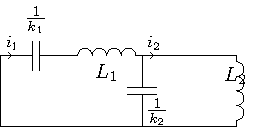
\includegraphics[width=\columnwidth]{2022/NM/54/figs/tikz.pdf}
    \caption{ }
    \label{fig:ishitha.g22.nm.54.f3}
\end{figure}  
 
\begin{align}
 k_1\int i_1 \, dt + L_1\frac{di_1}{dt}+k_2\int \brak{i_1-i_2} \, dt &=0
\label{eq:ishitha.g22.nm.54.5.eq} \\
 L_2\frac{di_2}{dt}-k_2\int \brak{i_1-i_2} \, dt &=0
\label{eq:ishitha.g22.nm.54.6.eq} 
\end{align}

but we know, $i=\frac{dq}{dt}$ 
 \begin{align}
 \implies L_1\ddot q_1 -k_2\brak{q_2-q_1} + k_1q_1  &=0 
 \label{eq:ishitha.g22.nm.54.7.eq} \\
 \implies L_2\ddot q_2+k_2\brak{q_2-q_1} \, dt &=0
  \label{eq:ishitha.g22.nm.54.8.eq}
\end{align}  


Writing ~\eqref{eq:ishitha.g22.nm.54.7.eq} and ~\eqref{eq:ishitha.g22.nm.54.8.eq} in matrix form:
\begin{align}
\myvec{
L_1 & 0  \\
0 & L_2
}
\myvec{
\ddot{q_1}(t) \\
\ddot{q_2}(t)
}
+
\myvec{
k_1+k_2 & -k_2  \\
-k_2 & k_2
}
\myvec{
q_1(t) \\
q_2(t)
}
=
\myvec{
0 \\
0
}
\end{align}

\begin{equation}
q(t)     \systemL{}   Q(s)  
\end{equation}


\begin{equation}
q^{''}(t) \systemL{} s^{2}Q(s)-sq(0)-q^{'}(0)
\end{equation}

Assuming charge to be maximum at t=0;
\begin{align}
L_1\brak{s^2Q_1(s)-sq_1(0)} - k_2\brak{Q_2(s)-Q_1(s)} + k_1Q_1(s) &= 0
\label{eq:ishitha.g22.nm.54.9.eq} \\
L_2\brak{s^2Q_2(s)-sq_2(0)} + k_2\brak{Q_2(s)-Q_1(s)}&=0
\label{eq:ishitha.g22.nm.54.10.eq} 
\end{align}

Writing ~\eqref{eq:ishitha.g22.nm.54.9.eq} and ~\eqref{eq:ishitha.g22.nm.54.10.eq} in matrix form:
\begin{align}
\myvec{
L_1s^2 + \brak{k_1+k_2} & -k_2  \\
-k_2& L_2s^2+k_2
}
\myvec{
Q_1(s) \\
Q_2(s)
}
=
\myvec{
L_1sq_1(0) \\
L_2sq_2(0)
}
\end{align}

\begin{align}
\myvec{
Q_1(s) \\
Q2(s)
}
= \frac{1}{L_1L_2s^4+(k_1+k_2)L_2s^2+k_2L_1s^2+k_1k_2} \nonumber \\
\myvec{
L_2s^2+k_2 & k_2  \\
k_2& L_1s^2 + \brak{k_1+k_2}
}
\myvec{
L_1sq_1(0) \\
L_2sq_2(0)
}
\end{align}

\begin{align}
\implies Q_1(s)&=\frac{L_1L_2s^3q_1(0)+k_2L_1sq_1(0)+k_2L_2sq_2(0)}{L_1L_2s^4+(k_1+k_2)L_2s^2+k_2L_1s^2+k_1k_2} \\
\implies Q_2(s)&= \frac{k_2L_1sq_1(0)+L_1L_2s^3q_2(0)+\brak{k_1+k_2}L_2sq_2(0)}{L_1L_2s^4+(k_1+k_2)L_2s^2+k_2L_1s^2+k_1k_2} 
\end{align}

Considering denominator of $Q_i(s)$ for $i=1,2$(ie: characteristic equation of the system):
\begin{align}
L_1L_2s^4+(k_1+k_2)L_2s^2+k_2L_1s^2+k_1k_2 &=0 \\
s^4 +4s^2+2&=0\\
\implies s^2&=\frac{-4\pm \sqrt{16-8}}{2} \\
&= -2 \pm \sqrt{2} 
\end{align}
The roots of s are imaginary so it's Sinusoid.
\begin{align}
\omega&=\pm\sqrt{2\mp \sqrt{2}}\\
\implies \omega_{least} &= 0.765 rad/s
\end{align} 

%\end{document}
